% Confidence-calibrated clarification for ask_and_confirm (RoBorregos home2 #1384)
% Build:  cd research/confidence_calibration && python run_all.py --data <dir>   (regenerates numbers)
%         cd paper && latexmk -pdf main.tex
\documentclass[10pt,a4paper]{article}
\usepackage[margin=2.2cm]{geometry}
\usepackage[T1]{fontenc}
\usepackage{lmodern}
\usepackage{amsmath,amssymb}
\usepackage{graphicx}
\usepackage{booktabs}
\usepackage{float}
\usepackage{xcolor}
\usepackage{caption}
\usepackage{subcaption}
\usepackage{tikz}
\usetikzlibrary{arrows.meta,positioning}
\usepackage[hidelinks]{hyperref}

\newcommand{\DataSource}{TTS voices transcribed by the robot Whisper (proxy)}
\newcommand{\IsSynthetic}{0}
\newcommand{\IsTTS}{1}
\newcommand{\FeatureList}{\texttt{conf\_mean}, \texttt{conf\_min}, \texttt{conf\_prod}, \texttt{conf\_whole\_mean}, \texttt{conf\_whole\_min}, \texttt{similarity}, \texttt{exact\_match}, \texttt{normalized\_flag}, \texttt{n\_words}, \texttt{n\_target\_words}, \texttt{avg\_logprob}, \texttt{no\_speech\_prob}}
\newcommand{\WOneAttempts}{771}
\newcommand{\WOneNormalized}{48}
\newcommand{\WOneNormalizedPct}{6.2\%}
\newcommand{\WOneZeroConf}{18}
\newcommand{\WOneZeroConfPct}{2.3\%}
\newcommand{\WOneFlipped}{26}
\newcommand{\WOneFlippedPct}{3.4\%}
\newcommand{\WOneFlippedWrong}{11}
\newcommand{\WOneLegacyOldAccept}{57.1\%}
\newcommand{\WOneLegacyFixAccept}{57.8\%}
\newcommand{\WTwoAttempts}{771}
\newcommand{\WTwoSpeakers}{41}
\newcommand{\WTwoCalibAttempts}{525}
\newcommand{\WTwoHeldAttempts}{246}
\newcommand{\WTwoCalibSpeakers}{29}
\newcommand{\WTwoHeldSpeakers}{12}
\newcommand{\WTwoErrorRate}{48.0\%}
\newcommand{\WTwoNameErrorRate}{47.5\%}
\newcommand{\WTwoDrinkErrorRate}{48.4\%}
\newcommand{\WTwoLabelSources}{intended: 771}
\newcommand{\WTwoTargetMet}{yes}
\newcommand{\WThreeSelected}{Logistic all + isotonic}
\newcommand{\WThreeAUROC}{0.83}
\newcommand{\WThreeAUROCLo}{0.74}
\newcommand{\WThreeAUROCHi}{0.92}
\newcommand{\WThreeECE}{0.090}
\newcommand{\WThreeLegacyAUROC}{0.68}
\newcommand{\WThreeLegacyECE}{0.295}
\newcommand{\WThreeMeanRawECE}{0.260}
\newcommand{\WThreeBestAUROC}{0.84}
\newcommand{\HOneVerdict}{supported}
\newcommand{\HTwoVerdict}{not supported}

\newcommand{\PolicyCostBonus}{15}
\newcommand{\PolicyCostWrong}{-40}
\newcommand{\PolicyCostMissing}{-40}
\newcommand{\PolicyRetries}{5}
\newcommand{\PolicySims}{30}
\newcommand{\PolicyMaxWrong}{18.9\%}
\newcommand{\PolicyMaxWrongRule}{the current heuristic's wrong-value rate plus 2 percentage points}
\newcommand{\TauBinaryAccept}{0.62}
\newcommand{\TauAccept}{0.52}
\newcommand{\TauRepeat}{0.50}
\newcommand{\HThreeConfirmReduction}{78.5\%}
\newcommand{\HThreeWrongDelta}{-6.8 pp}
\newcommand{\HThreeScoreLegacy}{-5.8}
\newcommand{\HThreeScoreBest}{-0.7}
\newcommand{\HThreeScoreAlways}{-9.5}
\newcommand{\HThreeVerdict}{supported}
\newcommand{\HThreeA}{yes}
\newcommand{\HThreeB}{yes}
\newcommand{\HThreeC}{yes}


\definecolor{warnbg}{HTML}{FDF1E9}
\definecolor{warnfg}{HTML}{9A3B12}
\newcommand{\code}[1]{\texttt{#1}}
% \input inside tabular breaks the booktabs rules; the TeX primitive does not
\makeatletter\newcommand{\inputrows}[1]{\@@input #1 }\makeatother

\title{Accept, Repeat or Confirm?\\
\large Confidence-Calibrated Clarification for Speech Slot Filling on a Service Robot}
\author{RoBorregos @Home -- HRI area}
\date{Issue \#1384 \quad Data: \DataSource}

\begin{document}
\maketitle

\ifnum\IsSynthetic=1
\begin{center}
\colorbox{warnbg}{\parbox{0.92\linewidth}{\color{warnfg}\small\textbf{Synthetic data.}
Every number in this version comes from \code{make\_synthetic.py}, a simulated dataset with the exact
format of the robot logs. It shows that the pipeline runs end to end. It is \emph{not} a result. Re-run
\code{run\_all.py -{}-data data} once the week-2 recordings are labeled.}}
\end{center}
\fi
\ifnum\IsTTS=1
\begin{center}
\colorbox{warnbg}{\parbox{0.92\linewidth}{\color{warnfg}\small\textbf{TTS proxy data.}
The audio is synthetic speech (edge-tts voices with 16 English accents, plus added noise and reverb),
but every word probability comes from the robot STT (\code{distil-large-v3}, same decoding settings).
The extraction LLM is emulated by rules. The numbers are a proxy for the week-2 human recordings, not a
replacement: TTS voices are more regular than people. Re-run \code{run\_all.py -{}-data data} with the
human sessions before shipping thresholds.}}
\end{center}
\fi

\begin{abstract}
FRIDA asks for a guest's name and favorite drink in the Human-Robot Interaction Challenge (HRIC). Before this
work, a fixed heuristic decided whether to accept the transcribed value or ask ``Did you say X?'': both the
Whisper word probability and the option similarity had to exceed $0.7$. The thresholds had never been measured,
and the 2027 rulebook rewards not asking such non-essential questions ($+15$) while penalizing every wrong
memorized value ($-40$). We instrument the dialog, fix a matching bug that set the confidence of normalized
values to zero, and replace the rule with a calibrated estimate of $p(\text{correct})$ that drives a three-way
policy: \emph{accept}, \emph{ask to repeat} (free under the rules) or \emph{confirm}. On held-out speakers, the
selected model (\WThreeSelected) reaches AUROC \WThreeAUROC{} [\WThreeAUROCLo, \WThreeAUROCHi] and ECE
\WThreeECE. The three-way policy changes confirmation questions by \HThreeConfirmReduction{} relative to
the current heuristic, changes the wrong-value rate by \HThreeWrongDelta{}, and moves the expected name/drink
score from \HThreeScoreLegacy{} to \HThreeScoreBest{} points per guest.
\end{abstract}

%=====================================================================
\section{Introduction}
Speech slot filling, such as ``What is your name?'', is the first point of contact in most @Home tasks. Two
errors cost points in opposite directions. A robot that accepts a misheard name stores wrong guest information
($4\times-40$ in HRIC). A robot that always asks ``Did you say X?'' loses the non-essential-question bonus
($4\times15$) and spends about 5\,s per question. The rulebook explicitly allows asking a guest to repeat
when the robot could not hear, and does not count it as a non-essential question~\cite{robocup2027rules}.
This creates a third option that the original implementation did not use. GPSR has a different trade-off: a
rephrasing request costs $-30$, but a misunderstood command loses both understanding ($80$) and solving
($250$).

\paragraph{Research question.} Do calibrated STT and extraction confidence signals allow a three-way policy
(accept / repeat / confirm) to reduce non-essential questions without increasing wrong memorized
information, compared to the current heuristic?

\paragraph{Hypotheses.}
\textbf{H1:} the confidence features predict extraction errors with AUROC $\ge 0.80$.
\textbf{H2:} after calibration, ECE $\le 0.05$.
\textbf{H3:} compared to the current heuristic, the calibrated policy (a) cuts confirmation questions by
$\ge 50\%$, (b) with $\le 2$ percentage points more wrong memorized values, and (c) a higher expected HRIC
score.

%=====================================================================
\section{Related work}
Modern neural networks are often over-confident, and post-hoc calibration such as temperature or Platt
scaling~\cite{platt1999probabilistic,guo2017calibration} or isotonic regression~\cite{zadrozny2002isotonic}
repairs the mapping from score to probability. Whisper~\cite{radford2023whisper} exposes per-word
probabilities that, as we show below, are not calibrated for short in-domain utterances. KnowNo~\cite{ren2023knowno}
calibrates when an LLM planner should ask for help, using conformal prediction. We apply the same idea, ``ask
only when the calibrated uncertainty warrants it'', to a much smaller decision with a known cost function, the
competition scoresheet.

%=====================================================================
\section{System and baseline (week 1)}
\label{sec:system}
\begin{figure}[t]
\centering
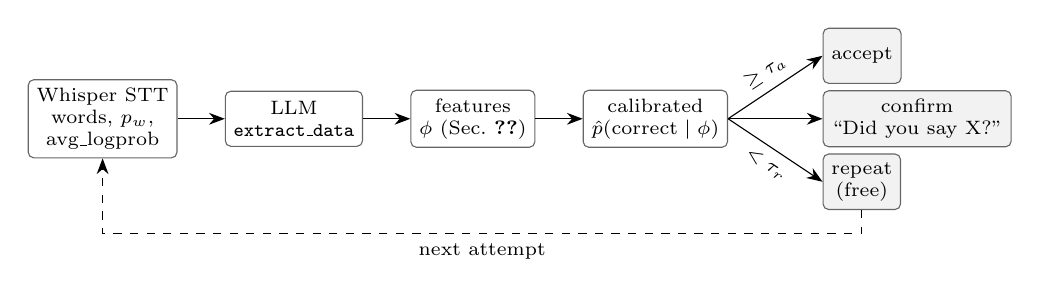
\begin{tikzpicture}[node distance=4mm and 6mm, every node/.style={font=\scriptsize},
  box/.style={draw=black!60, rounded corners=2pt, align=center, minimum height=7mm, inner sep=3pt},
  dec/.style={box, fill=black!5}, >={Stealth[length=2mm]}]
\node[box] (stt) {Whisper STT\\words, $p_w$,\\avg\_logprob};
\node[box, right=of stt] (llm) {LLM\\\code{extract\_data}};
\node[box, right=of llm] (feat) {features\\$\phi$ (Sec.~\ref{sec:features})};
\node[box, right=of feat] (cal) {calibrated\\$\hat p(\text{correct}\mid\phi)$};
\node[dec, right=12mm of cal, yshift=8mm] (acc) {accept};
\node[dec, right=12mm of cal] (conf) {confirm\\``Did you say X?''};
\node[dec, right=12mm of cal, yshift=-8mm] (rep) {repeat\\(free)};
\draw[->] (stt) -- (llm); \draw[->] (llm) -- (feat); \draw[->] (feat) -- (cal);
\draw[->] (cal.east) -- node[above, sloped]{$\ge\tau_a$} (acc.west);
\draw[->] (cal.east) -- (conf.west);
\draw[->] (cal.east) -- node[below, sloped]{$<\tau_r$} (rep.west);
\draw[->, dashed] (rep.south) |- ++(0,-3mm) -| node[pos=0.25, below]{next attempt} (stt.south);
\end{tikzpicture}
\caption{Decision pipeline of \code{HRITasks.ask\_and\_confirm}. Every attempt writes one JSONL record
(\code{logs/hri\_decisions/}) with the transcription, word probabilities, features, decision and the user's
answer.}
\label{fig:pipeline}
\end{figure}

\paragraph{Baseline.} The original implementation averaged the Whisper probability of the words of the
extracted value and accepted when this mean and the option similarity were both above $0.7$, or when the value
matched an option exactly. Otherwise it confirmed.

\paragraph{Normalization bug.} For HRIC, name and drink are extracted by an LLM without an option list, so the
similarity is always $1$ and only the confidence matters. When the LLM normalizes the value (``coke'' $\to$
``Coca-Cola''), none of its words appear in the transcription. The matched set is then empty, the confidence
becomes $0$, and the robot always confirms. In the dataset, \WOneNormalized{} of \WOneAttempts{} attempts
(\WOneNormalizedPct) have a normalized value, and \WOneZeroConf{} (\WOneZeroConfPct) get a legacy confidence of
exactly $0$. We now fall back to the closest fuzzy span of the transcription, and to the whole transcription
when no span is close enough. This changes the legacy decision in \WOneFlipped{} attempts
(\WOneFlippedPct), \WOneFlippedWrong{} of which are wrong values that the bug was ``protecting''. The legacy
acceptance rate goes from \WOneLegacyOldAccept{} to \WOneLegacyFixAccept. The fix therefore removes an
arbitrary failure, but it also shows that the raw Whisper score is not a safe acceptance signal by itself.

\paragraph{Instrumentation.} \code{confidence\_policy.py} is a ROS-free module (unit tested with mocks) that
computes the features, applies the policy and writes the decision log. \code{CONFIDENCE\_POLICY} in
\code{hri\_constants.py} selects \code{legacy} (default, unchanged behavior), \code{binary} or \code{three\_way}.
The STT microservice now also returns the segment \code{avg\_logprob} and \code{no\_speech\_prob}.

%=====================================================================
\section{Method}
\subsection{Features}
\label{sec:features}
For the extracted value $v$ with matched word probabilities $p_1..p_k$: mean, minimum and product of $p_i$;
mean and minimum over the whole transcription; option similarity; exact-match flag; normalized-value flag
($v$ not a substring of the transcription); number of words of the transcription and of $v$; and, when
available, Whisper \code{avg\_logprob} and \code{no\_speech\_prob}. Features used: \FeatureList.

\subsection{Calibration}
We fit, on the calibration speakers only: isotonic regression on the mean or minimum confidence, Platt
scaling on the mean, and an $L_2$ logistic regression on all features (with an optional isotonic layer on its
out-of-fold scores). The model is selected by speaker-grouped 5-fold cross-validated log-loss on the
calibration split. The held-out speakers are used only for the final numbers. We report AUROC (95\% CI from a
speaker-level cluster bootstrap), ECE with 10 equal-width bins, and the Brier score. The selected model is
exported as JSON and evaluated on the robot by the same code (\code{CalibratedModel}), so no scikit-learn is
needed on board.

\subsection{Three-way policy}
Given $\hat p$: accept if $\hat p\ge\tau_a$; ask to repeat if $\hat p<\tau_r$ (except on the last attempt,
which confirms); otherwise confirm. The thresholds maximize the expected score per slot on the calibration
split:
\begin{equation}
  S = \PolicyCostBonus\cdot\mathbb{1}[\text{no confirmation}] \; \PolicyCostWrong\cdot\mathbb{1}[\text{wrong value}]
      \; \PolicyCostMissing\cdot\mathbb{1}[\text{no value after \PolicyRetries{} attempts}],
\end{equation}
subject to a wrong-value rate $\le$ \PolicyMaxWrong{} (\PolicyMaxWrongRule). The cost of a missing value is
our assumption: without a name or drink the later introduction items are lost. GPSR uses its own costs
($-30$ per rephrase, $-330$ per misunderstood command).

\paragraph{Offline replay.} Data is collected with \code{always\_confirm=True}, so every attempt has a label
and the user's yes/no. A policy is replayed slot by slot. When it needs another attempt (after a ``no'' or a
repeat), we use the next logged attempt of that slot. If there is none, we draw a random attempt of the same
speaker and slot (\PolicySims{} replays). This counterfactual assumes that repeating gives an exchangeable
new sample, which is optimistic if a speaker is consistently misheard.

%=====================================================================
\section{Dataset (week 2)}
Protocol: \code{collect\_confidence\_session.py} runs only the name/drink dialog with confirmation forced.
For each trial it prints a target value (25\% outside the official lists), which the speaker says in their own
words. Speaker id and condition (accent, noise, distance) are stored in every record. Labels come from
\WTwoLabelSources{} (a human label overrides the automatic one). Split by speaker: \WTwoCalibSpeakers{}
calibration speakers (\WTwoCalibAttempts{} attempts) and \WTwoHeldSpeakers{} held-out speakers
(\WTwoHeldAttempts{} attempts).

\ifnum\IsTTS=1
\paragraph{TTS proxy collection.} Until the human sessions exist, \code{make\_tts\_dataset.py} follows the same
protocol with synthetic speakers. Each edge-tts English voice is one speaker with a fixed condition: noise
(quiet, music, crowd babble made of other voices, or fan), a base SNR of 20, 10 or 5\,dB, and a distance of
0.5, 1.5 or 3\,m. Distance is simulated by an exponential reverb tail (RT$_{60}$ 0.25--0.8\,s) and a lower
SNR. Each attempt picks a new phrasing and speaking rate, and 60\% of Coca-Cola, Sidral Mundet and orange
juice targets are said as ``coke'', ``sidral'' or ``OJ''. The audio goes through faster-whisper with the robot
settings and the hotwords and initial prompt of the HRIC dialog. The extraction LLM is replaced by rules
that strip carrier phrases and normalize those aliases, exactly the case behind the normalization bug.
Labels are exact because the intended value is known.
\fi

\begin{table}[H]
\centering\small
\begin{tabular}{lrr}
\toprule
Condition & Attempts & Wrong value \\
\midrule
\inputrows{generated/conditions_table.tex}
\bottomrule
\end{tabular}
\caption{\WTwoAttempts{} labeled attempts from \WTwoSpeakers{} speakers (target $\ge200$ / $\ge10$:
\WTwoTargetMet). Overall error rate \WTwoErrorRate{} (name \WTwoNameErrorRate, drink \WTwoDrinkErrorRate).
A speaker contributes to several condition rows.}
\end{table}

\begin{figure}[H]
\centering
\begin{subfigure}{0.48\linewidth}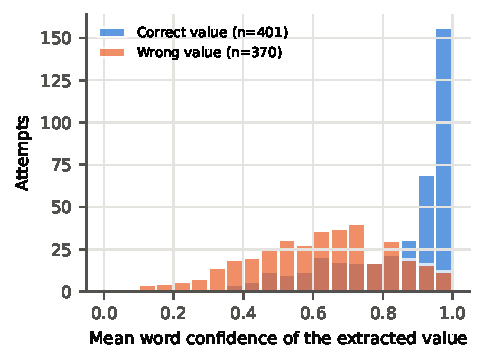
\includegraphics[width=\linewidth]{figures/hist_conf_mean.pdf}\end{subfigure}
\hfill
\begin{subfigure}{0.48\linewidth}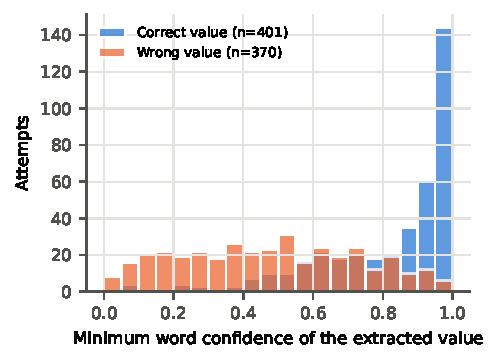
\includegraphics[width=\linewidth]{figures/hist_conf_min.pdf}\end{subfigure}
\caption{Whisper confidence of the extracted value for correct and wrong values. The overlap is the reason a
single fixed threshold cannot separate them.}
\end{figure}

%=====================================================================
\section{Results (week 3)}
\subsection{Calibration}
\begin{table}[H]
\centering\small
\begin{tabular}{lccc}
\toprule
Score / model (held-out speakers) & AUROC [95\% CI] & ECE & Brier \\
\midrule
\inputrows{generated/calibration_table.tex}
\bottomrule
\end{tabular}
\caption{Error prediction on held-out speakers. ``Raw'' rows use the Whisper score directly as a probability.
The bold model was selected on the calibration split.}
\label{tab:calibration}
\end{table}

\begin{figure}[H]
\centering
\begin{subfigure}{0.48\linewidth}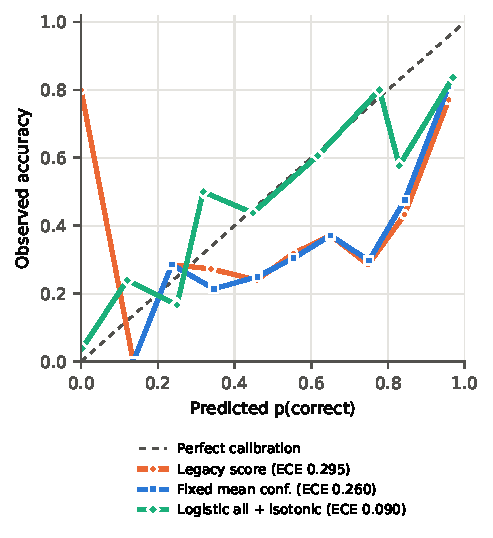
\includegraphics[width=\linewidth]{figures/reliability.pdf}\caption{Reliability}\end{subfigure}
\hfill
\begin{subfigure}{0.48\linewidth}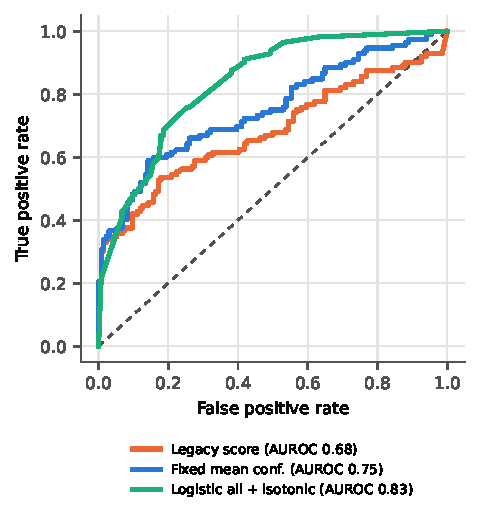
\includegraphics[width=\linewidth]{figures/roc.pdf}\caption{ROC}\end{subfigure}
\caption{Held-out reliability diagram and ROC. The legacy score has ECE \WThreeLegacyECE{}, and the fixed raw
mean has ECE \WThreeMeanRawECE{}.}
\end{figure}

\subsection{Policy comparison}
\begin{table}[H]
\centering\small
\setlength{\tabcolsep}{4pt}
\begin{tabular}{lrrrrrrr}
\toprule
Policy & Wrong & Confirm/guest & Repeat/guest & Turns/slot & s/slot & No value & Points/guest \\
\midrule
\inputrows{generated/policy_table.tex}
\bottomrule
\end{tabular}
\caption{Offline replay on held-out speakers (2 slots per guest). Thresholds: binary $\tau_a=\TauBinaryAccept$;
three-way $\tau_a=\TauAccept$, $\tau_r=\TauRepeat$. Points count only the name/drink items
($+\PolicyCostBonus$ / $\PolicyCostWrong$).}
\label{tab:policy}
\end{table}

\begin{figure}[H]
\centering
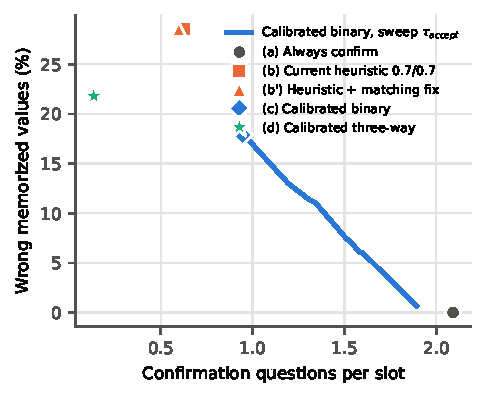
\includegraphics[width=0.55\linewidth]{figures/tradeoff.pdf}
\caption{Trade-off between non-essential questions and wrong memorized values on held-out speakers.}
\end{figure}

%=====================================================================
\section{Discussion}
\paragraph{Hypotheses.}
\textbf{H1} (AUROC $\ge0.80$): \HOneVerdict{} (AUROC \WThreeAUROC{}, CI [\WThreeAUROCLo, \WThreeAUROCHi]).
\textbf{H2} (ECE $\le0.05$): \HTwoVerdict{} (ECE \WThreeECE{}, versus \WThreeLegacyECE{} for the raw legacy
score).
\textbf{H3}: \HThreeVerdict{}. Confirmation questions changed by \HThreeConfirmReduction{} ($\ge50\%$:
\HThreeA), wrong values changed by \HThreeWrongDelta{} ($\le2$\,pp: \HThreeB), and expected points went
from \HThreeScoreLegacy{} to \HThreeScoreBest{} per guest (higher: \HThreeC). Always confirming scores
\HThreeScoreAlways.

\paragraph{What the scoresheet implies.} With $+15$ for not asking and $-40$ for a wrong value, accepting
pays off whenever $p(\text{correct}) > 40/55 \approx 0.73$, but only if $p$ is calibrated. A raw Whisper
probability of $0.7$ does not mean 70\% correct (Table~\ref{tab:calibration}). The free repeat is most useful
at low $\hat p$, where a confirmation question would most likely be answered ``no'' anyway.

\ifnum\IsTTS=1
\paragraph{TTS proxy caveats.} The error rate (\WTwoErrorRate) is far above what we expect from people at the
robot: the crowd and 3\,m conditions are harsh, and English TTS voices mispronounce Spanish and Yoruba targets
(``sidral'', ``Ximena'', ``Oluwaseun''). Names are labeled correct when their metaphone code matches, because
the robot says the name aloud (Adel / Adele, Mohammed / Muhammad); this also accepts Simone / Simon. When
$\tau_a \approx \tau_r$, the three-way policy almost never confirms: a free repeat beats a $-15$ confirmation,
at the price of more slots with no value after all attempts (Table~\ref{tab:policy}). Whether people tolerate
repeated ``could you repeat?'' prompts is a question for the live validation.
\fi

\paragraph{Limitations.} (i) The dataset is small\ifnum\IsTTS=1{} and synthetic in its audio\else{} and comes
from one robot and microphone\fi. The bootstrap CIs over speakers are wide. (ii) The repeat counterfactual assumes exchangeable attempts. (iii) Whisper
calibration depends on language, accent and hotwords, so the model must be refit when the STT model or
prompt changes. (iv) LLM extraction errors with confident STT, such as a wrong name chosen from a sentence,
are invisible to these features. This motivates the follow-up issue on LLM uncertainty (multi-sample
consistency or logprobs).

%=====================================================================
\section{Conclusion}
\ifnum\IsSynthetic=1
The instrumentation, the bug fix, the policy and the full evaluation pipeline are implemented and tested.
The numbers above come from simulated data and must not be quoted. The conclusion of this study will be
written from the week-2 recordings by re-running \code{run\_all.py}. Until then, the robot keeps
\code{CONFIDENCE\_POLICY = "legacy"} (with the matching fix).
\else\ifnum\IsTTS=1
On the TTS proxy data (\WTwoAttempts{} attempts, \WTwoSpeakers{} voices), with real Whisper probabilities,
H1 is \HOneVerdict, H2 is \HTwoVerdict{} and H3 is \HThreeVerdict. The calibrated three-way policy moves the
expected name/drink score from \HThreeScoreLegacy{} to \HThreeScoreBest{} points per guest, with a
\HThreeConfirmReduction{} reduction in confirmation questions and a \HThreeWrongDelta{} change in wrong
memorized values ($\tau_a=\TauAccept$, $\tau_r=\TauRepeat$). These numbers are provisional: they show the
direction of the effect with the real STT model, not its size with human speakers. The robot keeps
\code{CONFIDENCE\_POLICY = "legacy"} until the week-2 recordings confirm them.
\else
Calibrating the Whisper and extraction signals turns the arbitrary 0.7/0.7 rule into a decision with known
risk. H1 is \HOneVerdict, H2 is \HTwoVerdict{} and H3 is \HThreeVerdict{}: the calibrated three-way policy
moves the expected name/drink score from \HThreeScoreLegacy{} to \HThreeScoreBest{} points per guest, with
a \HThreeConfirmReduction{} reduction in confirmation questions and a \HThreeWrongDelta{} change in wrong memorized
values. The policy ships behind \code{CONFIDENCE\_POLICY="three\_way"}, with $\tau_a=\TauAccept$ and
$\tau_r=\TauRepeat$.
\fi\fi

\paragraph{Reproducibility.} Code: \code{task\_manager/utils/confidence\_policy.py},
\code{research/confidence\_calibration/}. \code{python run\_all.py -{}-data data} regenerates every number,
table and figure in this document from the logs.

\bibliographystyle{plain}
\bibliography{refs}
\end{document}
